\documentclass[useAMS,usenatbib,usegraphicx]{mn2e} 
%=========================================================================
\usepackage{amsmath} 
\usepackage{amssymb} 
\usepackage{graphicx}
\usepackage{grffile}
\usepackage[dvips]{epsfig}
\usepackage{epsfig}  
\usepackage{color}
\usepackage{hyperref}
\newcommand{\apj}{ApJ}  
\newcommand{\jcap}{JCAP}  
\newcommand{\apjs}{ApJS}  
\newcommand{\pasa}{PASA}  
\newcommand{\apjl}{ApJL}  
\newcommand{\aj}{AJ}  
\newcommand{\mnras}{MNRAS}  
\newcommand{\mnrassub}{MNRAS accepted}  
\newcommand{\aap}{A\&A}  
\newcommand{\aaps}{A\&AS}  
\newcommand{\araa}{ARA\&A}  
\newcommand{\nat}{Nature}  
\newcommand{\physrep}{PhR}
\newcommand{\pasp}{PASP}    
\newcommand{\pasj}{PASJ}    
\newcommand{\hMpc}{{\ifmmode{h^{-1}{\rm Mpc}}\else{$h^{-1}$Mpc}\fi}}  
\newcommand{\Mpc}{{\ifmmode{{\rm Mpc}}\else{Mpc}\fi}}  
\newcommand{\hMsun}{{\ifmmode{h^{-1}{\rm{M_{\odot}}}}\else{$h^{-1}{\rm{M_{\odot}}}$}\fi}}
\newcommand{\Msun}{{\ifmmode{{\rm{M_{\odot}}}}\else{${\rm{M_{\odot}}}$}\fi}}
\newcommand{\kms}{{\ifmmode{{\rm{km\ s}^{-1}}}\else{km $\rm{s}^{-1}$}\fi}}


\begin{document}

%=========================================================================
%		FRONT MATTER
%=========================================================================
\title[LG satellite alignments]{Local Group Satellite Alignments}
\author[J.E. Forero-Romero \& V. Arias]
{Jaime E. Forero-Romero $^{1}$ \thanks{je.forero@uniandes.edu.co},
Ver\'onica Arias$^1$\\
%%
$^1$ Departamento de F\'isica, Universidad de los Andes, Cra. 1
  No. 18A-10 Edificio Ip, CP 111711, Bogot\'a, Colombia \\
}

\maketitle

\begin{abstract}
We focus on the spatial distribution of bright ($M_V<-8$) satellites and
pairs of galaxies with similar masses, isolation and kinematic
configurations as the Local Group. 
\end{abstract}

\begin{keywords}Galaxies: halos --- Galaxies: high-redshift --- Galaxies: statistics
--- Dark Matter --- Methods: numerical 
\end{keywords}

\section{Introduction}

\section{Observational Characterists of Andromeda and the Milky Way}
\label{sec:obs}


\section{Local Group Analogues in the Illustris Simulation}
\label{sec:NumericalSetup}

We use publicly available data from the Illustris Project 
\citep{2014MNRAS.444.1518V}. 
This suite of cosmological simulations, performed using the quasi-Lagrangian
code AREPO \citep{2010MNRAS.401..791S}, follow the coupled evolution of dark 
matter and gas and includes parametrizations to account for the effects of
gas cooling, photoionization, star formation, stellar feedback, black
hole and super massive black hole feedback. 

The simulation volume is a cubic box of $75$ \hMpc\ on a side.
The cosmological parameters correspond to a $\Lambda$CDM cosmology
consistent with WMAP-9 measurements \citep{2013ApJS..208...19H}. 

We extract halo and galaxy information from the Illustris-1 simulation
which has the highest resolution in the current release of the
Illustris Project.
Illustris-1 has $1820^3$ dark matter particles and $1820^3$ initial gas
volumen elements. 
This corresponds to a dark matter particle mass of
$6.3\times 10^6$\Msun\ and a minimum mass for the baryonic volume
element of $8.0\times 10^7$\Msun. 
The corresponding spatial resolution is $1.4$ kpc for the dark matter
gravitational softening and $0.7$ kpc for the typical size of the
smallest gas cell size. 

We compute the cosmic web from the DM information in the
Illustris-3 simulation which share the same structure information with
Illustris-1 on scales of $1$ \Mpc.  
Illustris-3 has $456^3$ DM particles, corresponding to
$4.0\times 10^8$ \Msun in DM particle mass and $5.7$ kpc for the DM
gravitational softwning lentgh.
 

\subsection{Sample Selection: Local Group Analogues}

We build a sample of Local Group Analgues (LGA) by performing a selection on
the stellar mass and isolation properties of the galaxies in the
simulation. The conditions to select LGA galaxies are the following.

\begin{itemize}
\item LGA galaxy pairs are composed by galaxies with stellar mass in the
range $1\times10^{10}\Msun <M_{\star}<1.5 \times 10^{11} \Msun$.
\item For each galaxy $A$ we find its closest galaxy $B$, if galaxy $A$ is also
the closest to halo $B$, the two halos are considered as a pair. 
Another way to phrase this selection is that pairs do not have
neighbors closer than the pair's separation.
\item The distance between the galaxies' center of
  mass must be in the range $500$ kpc $<d_{AB}<$ $1500$ kpc. 
\item For each galaxy in the pair there cannot be a galaxy more
  massive than the lightest galaxy in the pair within a radius of $2$
  Mpc. 
\end{itemize}

We find $19$ pairs with these conditions.
Figure \ref{fig:samples} shows the radial velocity versus distance for
the LGA pairs.

\begin{figure}
\centering
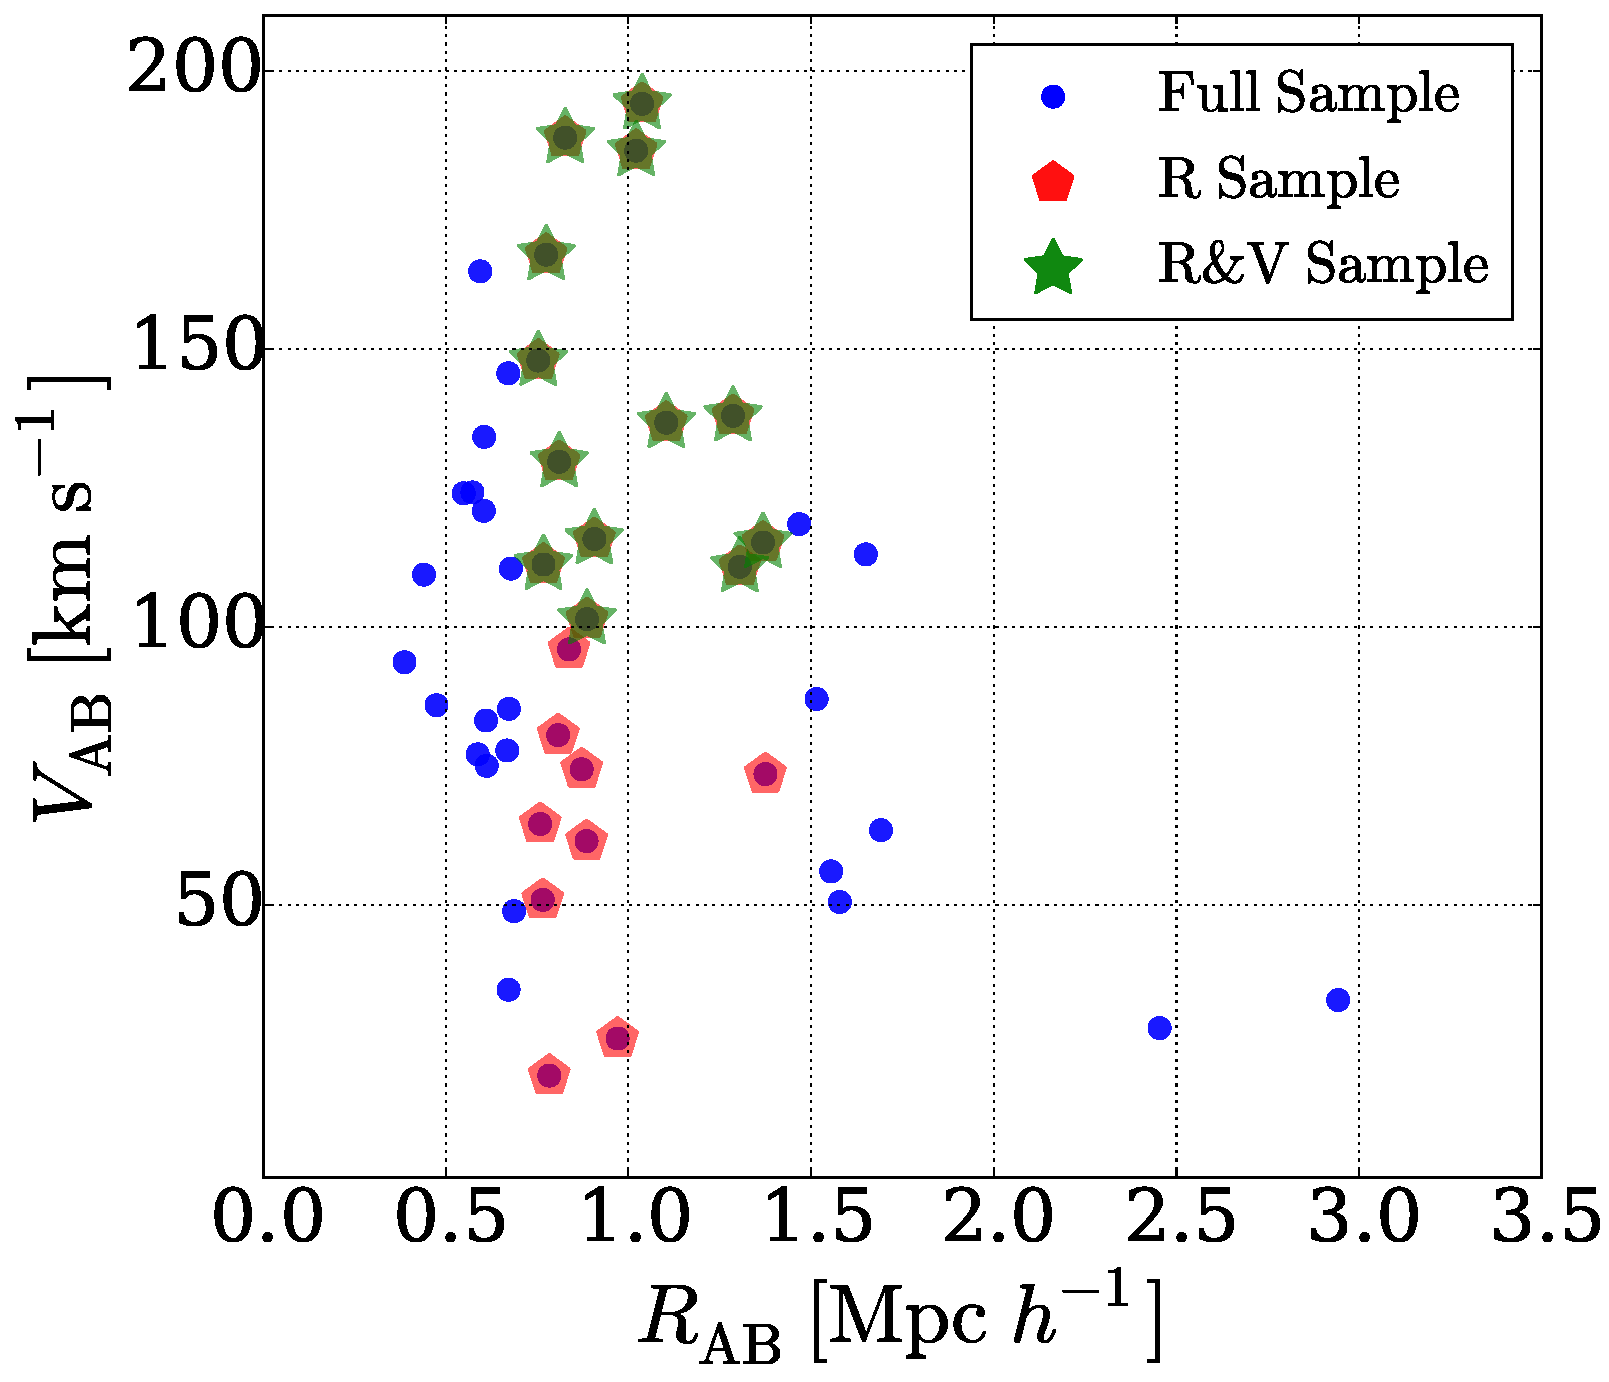
\includegraphics[width=0.5\textwidth]{v_r_pairs.pdf}
\caption{Halo pair samples used in this paper located in the
  plane of relative radial velocity $V_{r,AB}$ versus 
  distance $R_{AB}$ between the two halos in the pair.
  The IP sample (24 pairs) is a general pair sample, while the LGP
  sample (12 pairs) resemples the separation and kinematic
  conditions observed in the Local Group.} 
\label{fig:samples}
\end{figure}


\section{Cosmic Web Calculations}
\label{sec:CosmicWeb}

We place the LGA pairs into the cosmic web as quantified by the
deformation tensor  
\citep{2007MNRAS.375..489H,2009MNRAS.396.1815F}.
This method computes a cartesian grid the tidal tensor 
\begin{equation}
T_{ij} \equiv \frac{\partial^2\phi}{\partial r_i \partial r_j},
\end{equation}
%
where $\phi$ is a pseudo-gravitational potential that satisfies the
Poisson equation $\nabla^2\phi=\delta$, with $\delta$ the DM matter
overdentisy, and the $r_i$ coordinates correspond to a cartesian
system with $i=1,2,3$.   

This tensor can be diagonalized.
Its eigenvalues ($\lambda_1 > \lambda_2 > \lambda_3$) and
corresponding eigenvectors ($\hat{e}_1$, $\hat{e}_2$, $\hat{e}_3$)
define the degree and direction of stability around the neighborhood
where the tensor is computed. 
This allows the classification of that region either as a peak,
filament, sheet or voids in the case of three, two, one or zero
eigenvalues larger than a given threshold $\lambda_{\rm th}$.

In this study we compute these eigenvalues and eigenvectors over the
dark matter component of the Illustris-3 simulation on a cubic mesh of
$74$ cells on a side. 
This resolution corresponds to $\sim 1$ \hMpc.
We interpolate the DM density on that mesh using a Cloud-In-Cell (CIC)
scheme, then smooth the density field with a gaussian window with a
physical scale equal to the cell size. 

We choose this interpolation and smoothing scale for two reasons.
First, because it corresponds to the typical pair separation in our
sample, making each halo in the pair share the same environment.
Second, because it allows a direct comparison with previous results in
the literature that used the same setup to quantify the cosmic
web environment for Local Group pairs in a cosmological context
\citep{ForeroRomero2013,2015ApJ...799...45F}.  

\section{Satellite Spatial Distribution and Alignment}
\label{sec:SpatialMeasurements}

We characterize the bright ($M_V<-9$) satellite spatial distribution
with four different metrics. 

\begin{enumerate}
\item{The inertia tensor}.
\item{Fitting planes}.
\item{Velocity Anisotropy}.
\item{Alignment with the cosmic web}. 
\end{enumerate}

I what follows we describe the details of implementation of each
metric.


\subsection{Inertia Tensor}
\label{sub:inertia}
First, by computing the inertia tensor defined as 

\begin{equation}
{\bf{\bar{I}}} = \sum_{k \in V}[(\bf{r}_i - \bf{r}_0)^2\cdot \bf{1} -
  (\bf{r}_i-\bf{r}_0)\cdot (\bf{r}_i - \bf{r}_0)^{T}],
\end{equation}
%
where $k$ indexes the set of satellites of interest
$\bf{r}_k$ are the satellites' positions, $\bf{r}_{0}$ is the
positions pof the host DM halo, $\bf{1}$ is the unit matrix,  and
${\bf r}^T$ is the transposed vector $\bf{r}$. 
We finally compute the eigenvalues, $a>b>c$, and corresponding
eigenvectors, $\hat{I}_a$, $\hat{I}_b$, $\hat{I}_c$, of this tensor.
In the case of a sheet-like configuration the vector perpendicular to
the sheet would be signaled by, $\hat{I}_a$, the eigenvector of the
largest eigenvalue. 

% referencia posiciones satellites
% http://adsabs.harvard.edu/abs/2013MNRAS.435.1928P

\subsection{Plane fitting}
\label{sub:planes}

We fit satellite planes around each galaxy in the pair by randomly
generating 10000 unit vectors over the  sphere, each vector
representing the direction perpendicular to a plane passing through
the main galaxy's center of mass. 
We compute the dot product of the unit vector with the position vector
for each satellite, this scalar gives us the satellite distance to the
plane. 
The best plane is determined by the vector that gives the lowest
position satellite distance dispersion. 
We take the dispersion value as a measure of the plane's width.
For comparison we store the value and direction giving the
highest distance dispersion.
We denote by $\hat{p}$ the unit vector defining the direction
perpendicular to the best plane.


\subsection{Velocity Anisotropy}
\label{sub:beta}

The velocity anisotropy paramenter, $\beta$ is defined as

\begin{equation}
  \beta = 1 - \frac{\sum_i v^2_{\rm{tan}; i}}{2\sum_i v^{2}_{\rm{rad};i}},
\label{eq:beta}
\end{equation}
% 
where $v_{\rm{tan/rad};i}$ correspond to the tangential/radial
velocity of the $i$-th satellite with respect to the central galaxy.



\begin{table*}
  \centering
\begin{tabular}{lll}
\hline\hline
Symbol & Units & Description\\\hline
$M_{\star}$ & $10^{10}$\Msun & Stellar mass of the central galaxy\\
$N_s$ & & Number of satellites with $M_V<-9$\\
$a > b> c$ & & Inertia tensor eigenvalues. \\
$\hat{I}_a$, $\hat{I}_b$, $\hat{I}_c$ & & Inertia tensor eigenvectors. \\
$\beta$  &  & Satellite Velocity Anisotropy\\
$\sigma_s$ & kpc & Plane width\\
$\lambda_1>\lambda_2>\lambda_3$ &  & Tidal tensor
eigenvalues\\
$\hat{e}_{1}$,  $\hat{e}_{2}$,  $\hat{e}_{3}$ &  & Tidal tensor
eigenvectors\\ 
$\hat{r}_{AB}$& & Unit vector in the direction to the galaxy companion\\
\hline\hline
\end{tabular}
  \caption{Overview of the parameters computed for each central galaxy
    and its satellite system.
  \label{tab:models}}
\end{table*}

\subsection{Cosmic Web Alignment}
\label{sub:webalignment}

\cite{2015ApJ...799...45F} showed tha LGA pairs present alignments
with the cosmic web.
The strongest alignment is between the eigenvector associated  with the smallest
eigenvalue, $\hat{e}_3$, and the vector $\hat{r}_{AB} $connecting the two halos in
the pair. 
The eigenvector $\hat{e}_3$ indicates the direction along
which the cosmic web filament lies and in the case of being on a local
sheet it is a vector lying on the pancakes' plane. 

Following \cite{2014MNRAS.443.1090F} we compute the closest cosmic web
eigenvalue  towards which the vectors $\hat{r}_{AB}$, $\hat{p}$ and
$\hat{I}_a$ are aligned. 

\bibliographystyle{mn2e}
\bibliography{Dwarfs}

%% Alignments between galaxies, satellite systems and haloes
%% https://arxiv.org/pdf/1605.01728.pdf

%% The tangential velocity excess of the Milky Way satellites
%% https://arxiv.org/pdf/1612.01529.pdf

%% Tambien deberiamos sacar las alineaciones con el momentum angular
%% de las estrellas de las galaxias principales.

%% http://adsabs.harvard.edu/abs/2017MNRAS.464.3825P
\end{document}

